\section{Technology}
\label{sec:background}

In this section we will go into detail about microservices architecture and how we used Thorntail to achieve this. We compare a microservice architecture to a traditional monolithic approach, to look at what you as a developer and your application can benefit from choosing a microservice architecture.

\subsection{Microservice Architecture}
The idea behind a microservice architecture is to split an application into a set of smaller, interconnected services. Each microservice functions as a small application and has its own architecture consisting of business logic and a communication technology. \\

\noindent One of the most prominent features of the microservice architecture pattern is how it affects the relationship between the application and the database. In a monolithic architecture its traditional to share one database schema across the entire application, but with microservices each service has its own database schema. This will probably lead to some duplication of data across the entire application, but it's necessary to ensure loose coupling between services. \\

\noindent Another important aspect of this architecture is that client applications don’t directly communicate with the back-end services. Instead clients requests/sends information from/to an API Gateway. The API Gateway is responsible for tasks such as load balancing, caching, access control, API metering and monitoring. \cite{MicroArticle}\\

\noindent A traditional monolithic architecture usually consist of a database, application back-end and client-side. Where most of the business logic is implemented in the back-end, all the data for the entire application is stored in one database schema and the client-side requests information directly from the back-end or a REST-api. At the beginning of the development phase this is easy to develop, deploy and scale, but as time goes this can change due to increasing complexity and code base. One of the biggest drawbacks for the monolithic architecture is that it usually means a long-term commitment to a technology stack. \cite{MonolithArch}

\subsection{Concepts}
The concepts focused on in this section is what is what a microservice architecture can do for the application and its developers in the long run. Even though the microservice architecture in the {figure above} seems far more complex than the monolithic architecture, we will do our best to show that the microservice approach brings a lot of benefits to both the application as a whole and its developers. \\
\newline
Each service should be independent of the rest of the system, and have its own database. The relative small codebase for each service makes the maintenance easier, and new developers will use less time to get an understanding of the codebase which he/she is working with. \\
\newline
Scalability in a microservice architecture is also worth mentioning. The fact that you can scale up one service at the time to reduce the response time for the system is also a major benefit to the monolithic approach, where you have to scale up the entire system. In other words, you can reduce the amount of overhead you have, and it ’s more cost efficient if you are looking at server costs.\\
\newline
In a monolithic application, you have to be aware that changes in some parts of the code can affect the entire codebase. On the other hand, when you want to expand a microservice application you severely limit the implications on the whole code base when you are changing a service, or adding a new one. \cite{MonolithArch} \\
\subsection{Thorntail}
Thorntail is a framework for creating small, standalone microservice-based applications, and is based on the WildFly Java application server. It claims to offer an innovative approach to packaging and running Java EE applications by producing just enough app-server. It does this through defining fractions[7] in the application’s pom.xml file. This ensures that the executable JAR doesn’t contain more functionality than it needs. \cite{ThorntailDoc}

\subsubsection{Uber- and Hollow JAR}
Thorntail offers two types of JARs. The uberjar is a single JAR file that includes everything you need to run your application. This includes both selected runtime components and the application components. This type of jar can be used for projects with continuous integration and continuous deployment pipelines, where a single executable binary artifact is produced and moved through the pipeline. The hollow JAR, on the other hand, removes the application components from the uberjar. This is meant for applications running on Linux containers such as Docker. When using containers you can add the runtime components to a container image below the application image in the hierarchy, this means that you can rebuild the application image faster if code changes appear.\cite{ThorntailDoc} 

\subsubsection{Logging}
Thorntail automatically enables logging through each of its fractions. This means, that by default you'll get logs that are service independent. Its also possible to define custom logging patterns in the \textit{project-defaults.yml}, as described in figure~\ref{fig:logging}. \cite{Thorntaillogging}\\

\begin{figure}[ht]
  \centering
  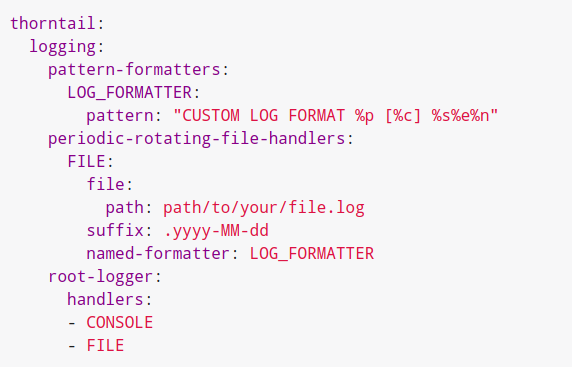
\includegraphics[scale=0.8]{figs/loggingconfig.png}
  \caption{Custom logging pattern to file}
  \label{fig:logging}
\end{figure}

\subsubsection{Distributed Tracing}
Thorntail makes it easy to debug through a process known as distributed tracing, even though an application is spread across multiple servers or instances. This is made possible through MicroProfile OpenTracing (cite something here), or another popular fraction, Jaeger (cite jaeger here). These APIs collects information about service invocations, correlating it to find all invocations related to a single user request, and visualizing the data in a form that enables easy debugging. This is also configurable through the \textit{project-defaults.yml} file in each service. \cite{ThorntailTracing}

\subsubsection{Metrics}
With this type of architecture, where a single user request invokes multiple services, diagnosing performance issues or reacting to service outages might be hard. Thorntail provides a fraction for providing metrics, namely MicroProfile Metrics. \cite{ThorntailMetrics} This enables developers to have information about:

\begin{itemize}
    \item How many requests are currently being processed
    \item How many connections to the database are currently in use
    \item How long service invocations take
\end{itemize}


